\chapter{Introduction}
\label{chapter:Introduction}


 
\section{Motivation}
\label{sec:intro}
One of the main challenges in robotics today is to bring robots into people's homes and make them help us to perform simple tasks. However, what we consider as a simple task might be very complex for an autonomous system. For example, when setting a table~\cite{iros10kcopman} the robot is likely to be
confronted with a cluttered unstructured scene\footnote{Following the discussion at the Clutter12
workshop at RSS 2012 we acknowledge that this is a ``laboratory clutter'' where the degree of difficulty
is similar to the scenes from the related works but still inferior to the real world clutter~\cite{matei2010manipulation}.} like the example shown
in \ref{fig:tracking_dists}. In order to interact with an environment like that a robot has to be able to detect and recognize the objects that are on the table. The main
motivation of this work is to show by leveraging robot's manipulation skills we can significantly improve its perception skills including segmentation and recognition of objects.
	
We can divide objects into three categories - textured, textureless and transparent with examples shown in Figure \ref{fig:all-objects}. In our work we address first two of them and we plan to focus on the third one in the future work.

\begin{figure}
%\centering

{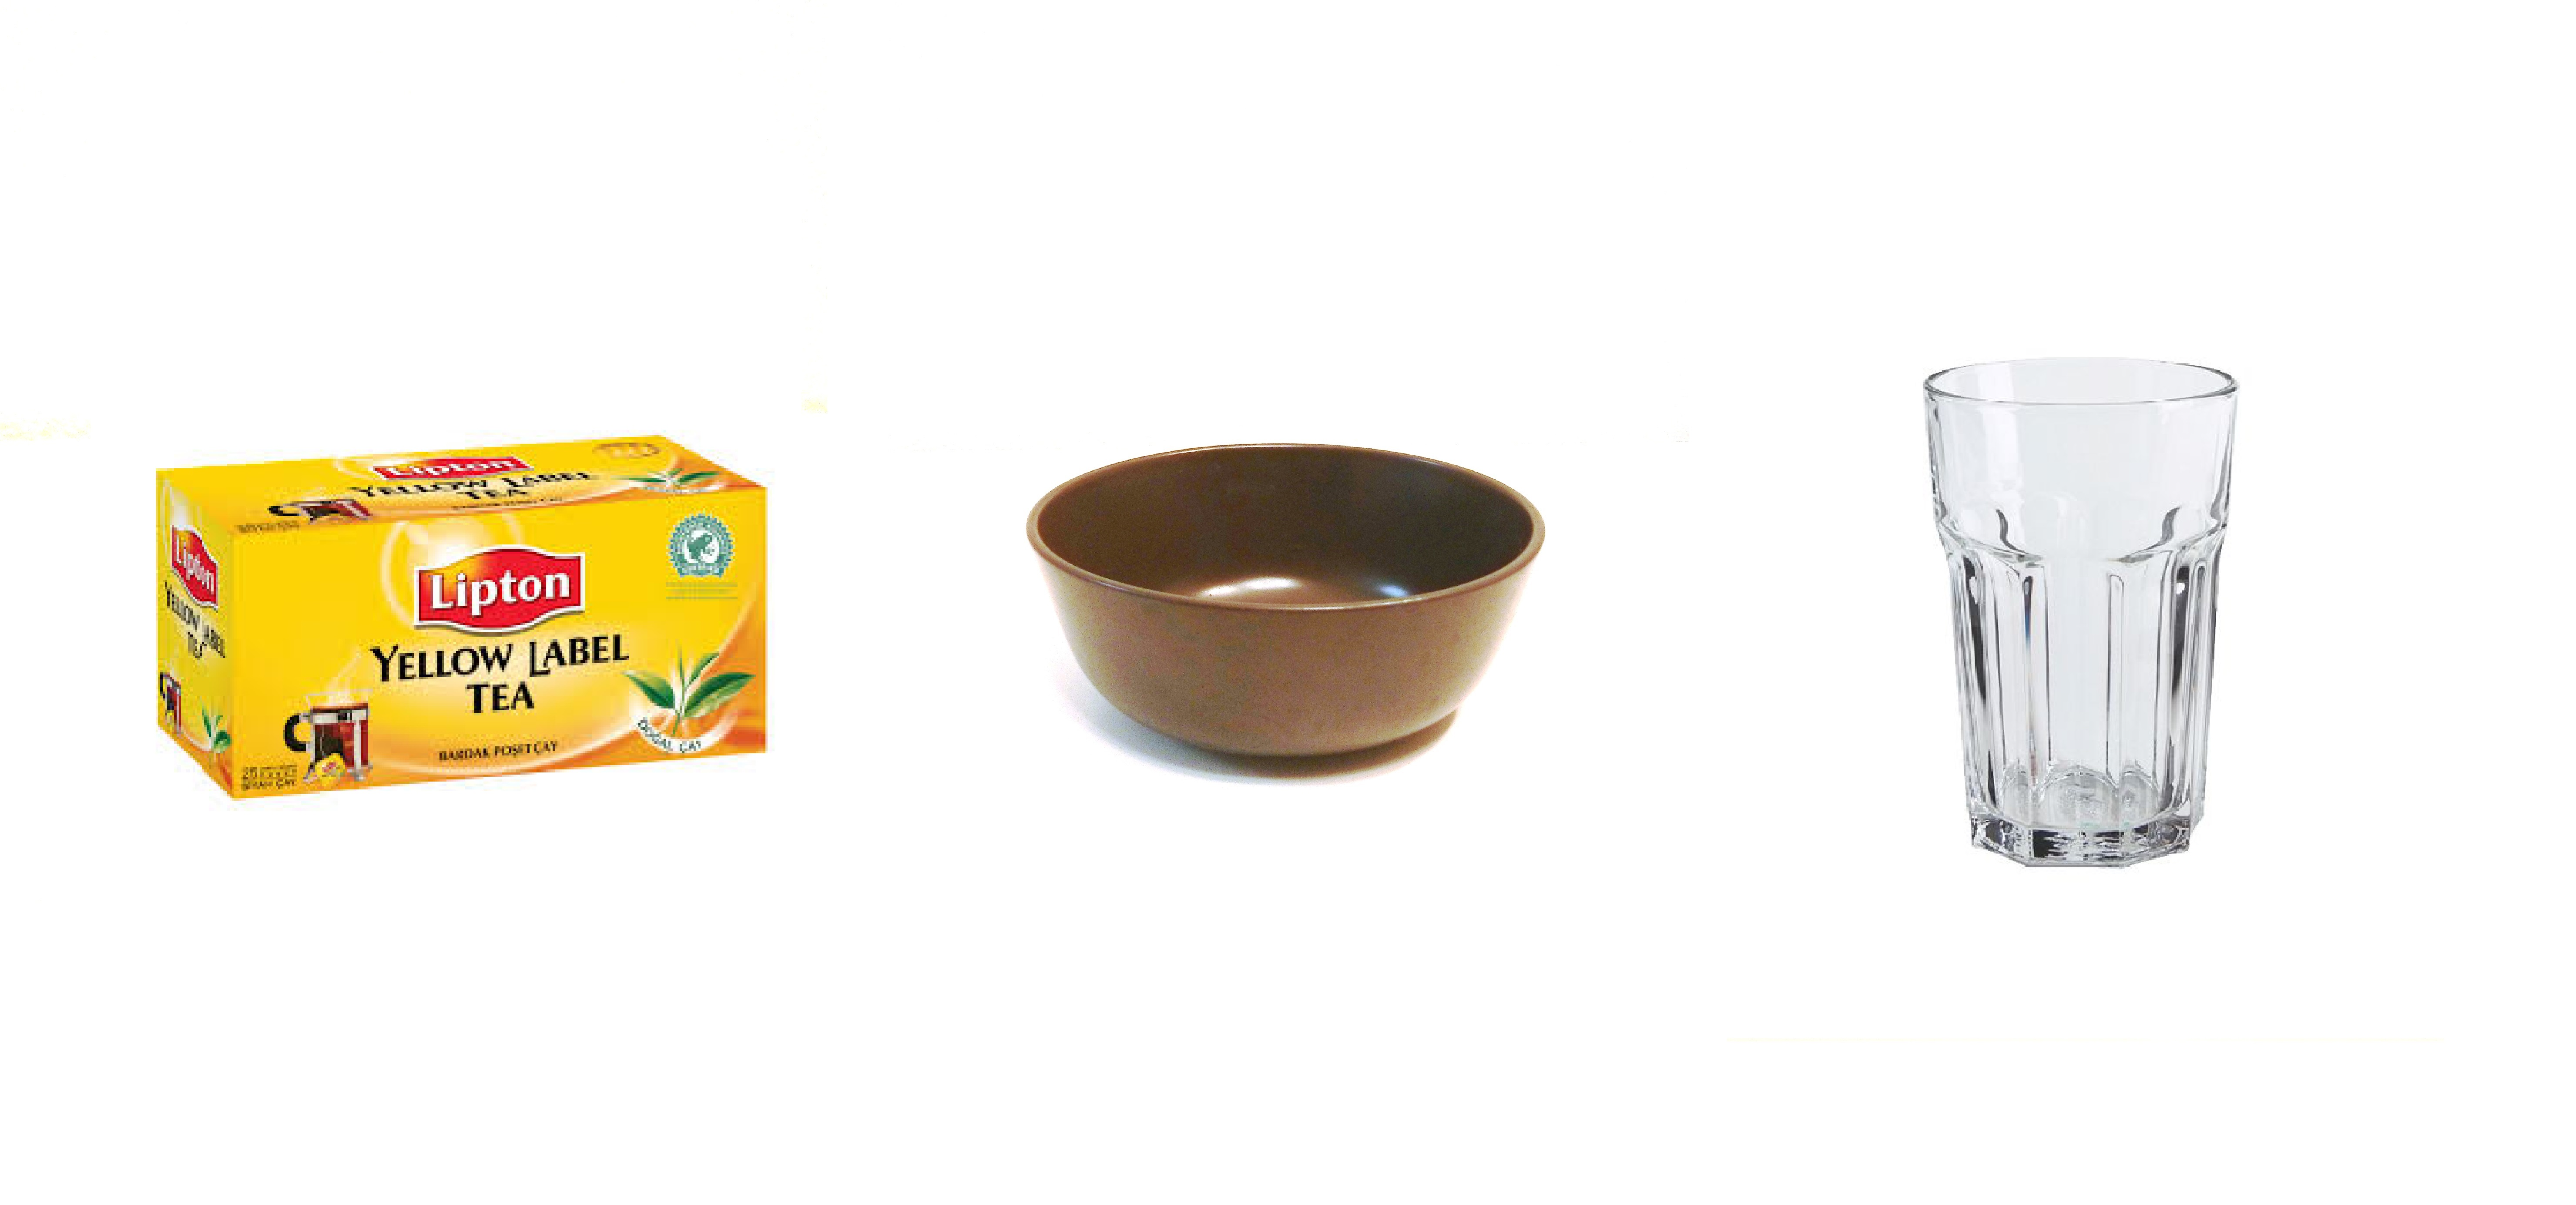
\includegraphics[width=1\columnwidth]{figures/all-objects.jpg}}

\caption{Three categories of objects: textured(left), textureless(middle), transparent(right)}
\label{fig:all-objects}
\end{figure}

As the initial step for the system we developed an interactive segmentation pipeline that is meant to be used for objects without any texture. In order to show that this is a challenging task that can not be solved with the state-of-the-art segmentation algorithms we refer reader to Figure \ref{fig:tracking_dists} where we tested three object segmentation algorithms that are used for segmentation of RGBD point clouds. Looking at the results we believe that the performance of robot's perception algorithms can be improved, especially in case of: 

\begin{itemize} 
\item textureless objects (all objects in the scene)
\item objects of the same color (a coffee mug and a saucer)
\item similar shape objects and occlusions (a white and a blue box);
\end{itemize}


In order to improve segmentation performance we decided to make use of robot's
capabilities. It is arguably more natural to exploit the robot's embodiment
and interaction capabilities in order to obtain a better understanding of its environment.
Reaching out to get a sense of what is around is the way how infants get to know their
``near space'' according to Piaget's theory~\cite{infants} of spatial cognition in the sensorimotor stage 
(until the age of 2), and getting a hold of connectivity (i.e. object unity) is an important
factor in the infant's understanding of objects at that stage.

\setlength{\tabcolsep}{0.1em}
\begin{figure}[ht]
%\centering
\begin{tabular}{cccc}
\multicolumn{2}{c}{\multirow{-6}{*}{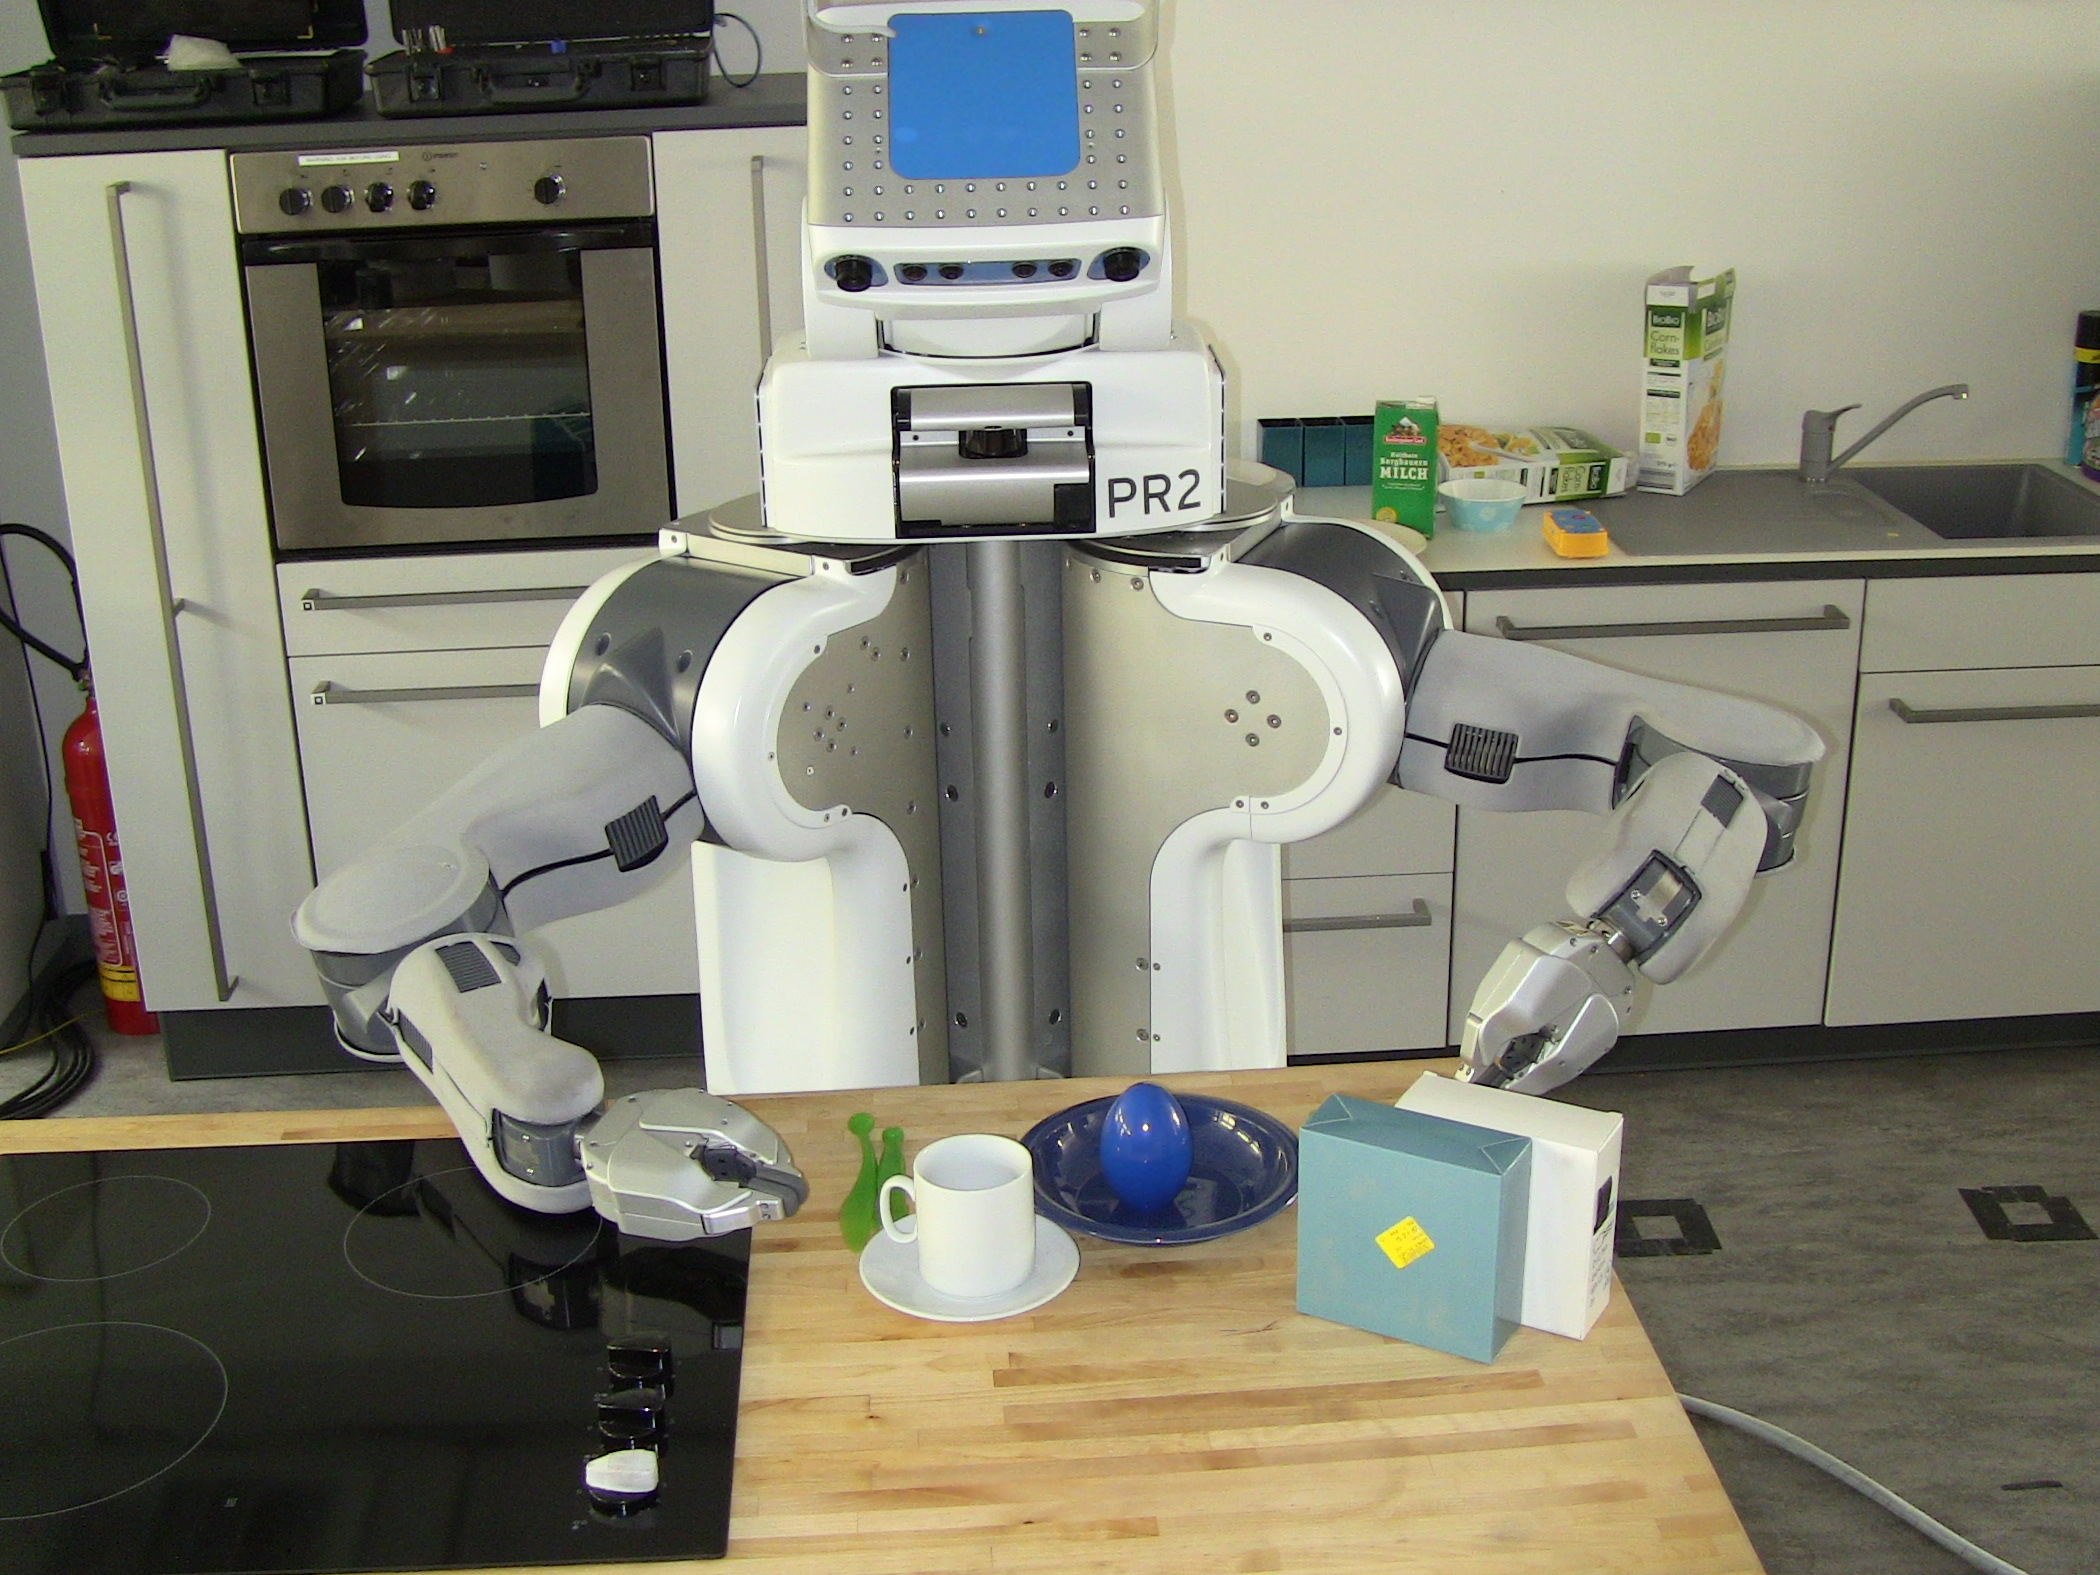
\includegraphics[width=0.5\columnwidth]{figures/teaser/IMG_0395.JPG}
}} & 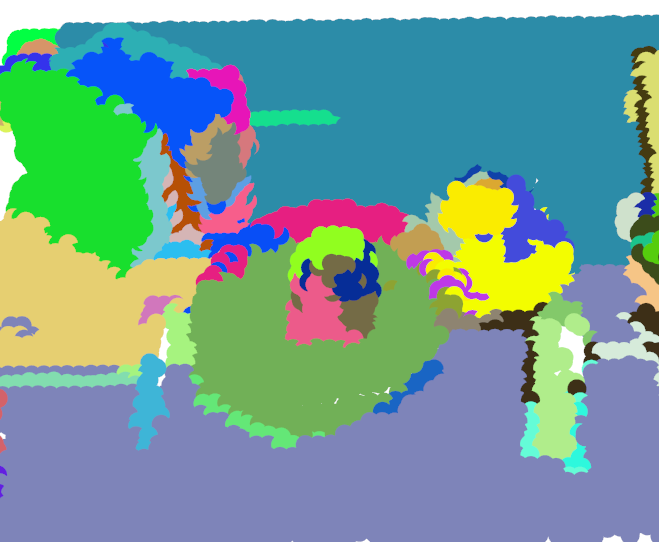
\includegraphics[width=0.23\columnwidth]{figures/segmentation_others/region_growing_rgb.png} 
&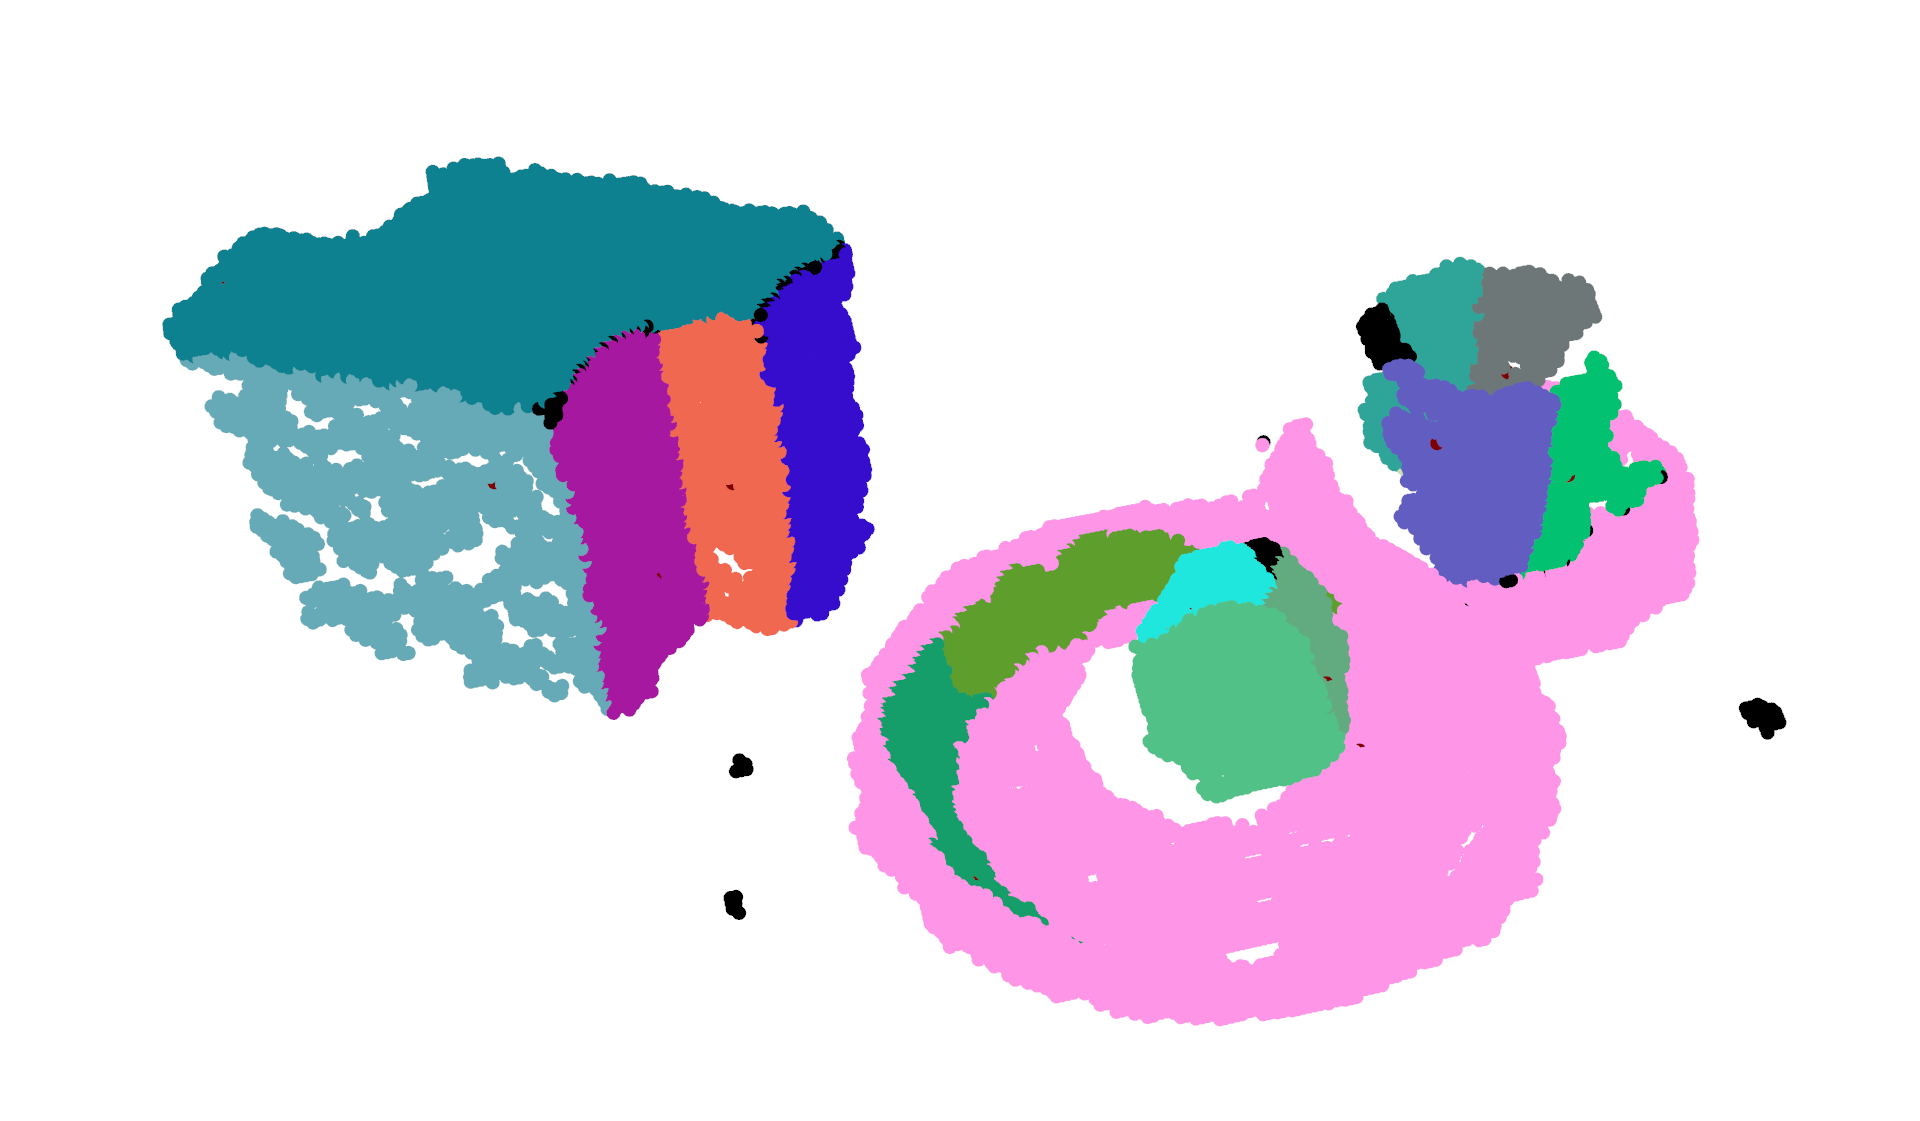
\includegraphics[width=0.23\columnwidth]{figures/segmentation_others/part-graph-hashing.png} \\
\multicolumn{2}{c}{} & \includegraphics[width=0.23\columnwidth]{figures/segmentation_others/graph-based.png} &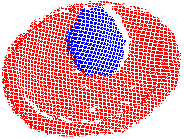
\includegraphics[width=0.23\columnwidth]{pictures/teaser_egg_result-cropped.png} 
%\multicolumn{2}{c}{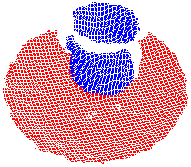
\includegraphics[width=0.38\columnwidth]{pictures/113-cropped.png}} 
\end{tabular}
\caption{Top-left: The service robot PR2 aiming to segment the scene
  consisting of textureless object. Results  of  the   scene segmentation
  using Region  Growing  method~\cite{RGBRegionGrowing} (top-right, NW), Part-Graph-based 
  Hashing~\cite{marton12SC} method (top-right, NE) and Graph-based  
  segmentation method~\cite{Felzenszwalb}   (top-right, SW). These methods work in depth, RGB and RGBD 
  space respectively and all underachieve due to the complexity of this challenging task. 
  On the other hand blue egg on the blue plate was correctly segmented using the interactive approach presented in this paper (top-right, SE)}
\label{fig:tracking_dists}
\end{figure}









\section{Problem definition and goals}

\subsection{Object Segmentation} 

In order to solve the challenge of object segmentation we need to define the terms - image segmentation and object, both in the sense of robot's perception. 


According to L.Shapiro and G. Stockman~\cite{shapiro2001computer}:

\noindent "Image segmentation is the process of partitioning a digital image into multiple segments. The goal of segmentation is to simplify and/or change the representation of an image into something that is more meaningful and easier to analyse."

\begin{figure}[ht]
%\centering
\begin{tabular}{cccc}

\multicolumn{2}{c}{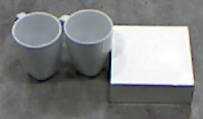
\includegraphics[width=0.45\columnwidth]{figures/3objects/after_push.jpg}}
& \multicolumn{2}{c}{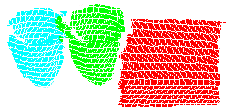
\includegraphics[width=0.45\columnwidth]{figures/3objects/segmented.png}}

\end{tabular}
\caption{Three white objects segmented correctly showing the generality of the apporach for multiple objects.}
\label{fig:three_objects}
\end{figure}


 Following this definition one can conclude that the goal of object segmentation is to segment the image in the way that it is partitioned into multiple objects. In our case we need to take into consideration that as an input we use point cloud data which is a natural extension of an image into 3 dimensional space. Therefore the same definition can be preserved for point clouds. 

A simple definition of an object in the sense of computer vision problem was presented by A. Mishra~\cite{mishra2012segmenting}:

\noindent "A simple object is defined as a compact region enclosed by the depth and
contact boundary in the scene".

According to this definition an output of the object segmentation algorithm is considered as multiple sets of points that form an object. That is, any point within the set belongs to that object's interior. 

As an example output of the object segmentation we refer reader to Figure \ref{fig:three_objects}. This Figure also shows that even though our experiments were conducted on the set of two objects, the algorithm is generic enough to handle multiple objects. In this context we understand objects as objects of daily use.


\subsection{Object Recognition}

Since the main terms are already defined we formulate the problem of object recognition. Once the object is segmented and the robot is aware of its boundaries it is crucial to be able to recognize which object it is. The statement of the object recognition is -  
given a database of objects and an image determine what, if any of the objects are present in the image. In this part of the thesis we concentrate on recognition of textured objects with the same idea that we used before - we leverage robot's manipulation capabilities in order to improve robot's perception.

In order to simplify the problem of model based recognition we constrain the region of interest such that the object is articulated. There are many systems in the field which came up with different solutions to the problem of reliable and robust object recognition. It is commonly believed that the most successful ones were the ones that were based on feature matching approach. All of them encountered to some extend the same problems, among others:

\begin{itemize}
\item features are not fully view point invariant, e.g. SIFT fails in case of larger than
$45^\circ$ rotation
\item  invariance to changing lighting conditions between the live
image and the one the object was trained on
\item image noise (lighting mentioned above)
\item large computational cost due to brute force matching;
\end{itemize}

The problem of object recognition can be understood much wider since we are entering the field of perceptual interpretation. Further implications that stem from information that database contains are not in the scope of this thesis.



\section{Approach} 

In this thesis we concentrate on solving two challenges: 

\begin{itemize} 
\item segmentation of textureless objects since the textured case was presented in~\cite{bersch12interactive} and~\cite{Katz-WS-MM-ICRA2011}

\item textured objects using interactive perception techniques.
\end{itemize} 

In the next subsections we concentrate on describing our approach for the above mentioned tasks.

\subsection{Interactive Segmentation of Textureless Objects} 


Starting from the object segmentation problem 
one we want to show that inducing the motion to the scene can solve the problems depicted in Figure \ref{fig:tracking_dists}. Similar  to Katz  et al.~\cite{Katz-WS-MM-ICRA2011}, Bergstrom et
al.~\cite{bergstrom11icvs}, and our earlier
work~\cite{bersch12interactive} we propose a system that uses
motion of robot's arm to enable effective
object  segmentation.

Our system consists of five main steps-being:

\begin{itemize} 
\item Static object pre-segmentation using part-graph-based hashing ~\cite{marton12SC}
\item Push point estimation using our previous work ~\cite{bersch12interactive}
\item Extraction of RGDB features using point cloud primitives such as lines, corners, cylinders and circles
\item Tracking of above mentioned features using Particle-Filter-based algorithm
\item Graph based trajectory clustering approach
\item Dense model reconstruction based on region growing in normal space;
\end{itemize} 


All of these steps are described in details in Chapter \ref{chapter:Textureless Segmentation}. 


There are three important assumptions in our system. First, that each item is a rigid  body and not subject
to large deformations when  interacting with  the robot's  end  effector or
other objects. We also assume that the objects are either flat (box-like) or round (cylinder-like),
which holds for most household objects in publicly available databases~\cite{marton11ijrr}, and
that in the tracking step the features do not get more than $50\%$ obstructed.

The evaluation was performed on 17 scenes with challenging arrangement of flat and
round objects of similar colors, shapes and sizes. $82\%$ of objects
were segmented correctly in these scenes. The interactive segmentation system is available online\footnote{\url{http://www.ros.org/wiki/interactive_segmentation_textureless}} with all instructions needed to install and run it on a real robot. The robot has to have a Kinect sensor as well as at least one arm in order to correctly use the system.

\subsection{Interactive Object Recognition} 

In the second challenge being object recognition we decided to build upon the approach presented in the segmentation system. Using our Interactive Segmentation pipeline we have a very good prior for the recognition of objects. Given that the object is segmented correctly we are able to constrain the problem of multiple object recognition to recognition of one currently segmented object at a time. In our system we show that even random rotations and translations can significantly improve recognition of objects.

In our approach we use the rotational movement of an object in order to eliminate the influence of view-point variance of features. We show that by incorporating robot's interaction with the environment we are also able to reduce the size of the database and thus, speed up the processing time of the algorithm.

In the chapter \ref{chapter:Object Recognition} we depict the problems and the initial solution in details as well as show promising results of our approach.
    















